\chapter{Introducción y Estado del Arte}

\section {Introducción}

La astronomía está atravesando una profunda transformación debido al desarrollo de modernos telescopios terrestres y satelitales, que han fomentado la realización de enormes relevamientos astronómicos \cite{Benjamin_2003} \cite{Skrutskie_2006} \cite{gaia} \cite{ogle}. Ante la abrumadora cantidad y calidad de los datos generados, se vuelve necesario el uso de procedimientos automatizados. Consecuentemente, diversas técnicas de aprendizaje automatizado y minería de datos surjen como una elección natural a la hora de analizar y extraer información de modernos datasets astronómicos. \cite{Richards_2011} \cite{303d9825f1794a8b86d692ee85c9a602}\\

\textit{Vista Variables in the Via Lactea (VVV)} es un relevamiento público del infrarrojo cercano que cubrió aproximadamente 520 $deg^2$ del disco y bulbo galáctico, utilizando el telescopio VISTA en Paranal, Chile \cite{vvv} (ver figura \ref{fig:vvv_telescope}). El VVV relevó aproximadamente $10^9$ fuentes astronómicas en las bandas ZYJHK durante un período de 5 años, teniendo entre sus principales objetivos la realización de un mapa tridimensional del bulbo galáctico. \\

\begin{figure}[h!]
\begin{center}
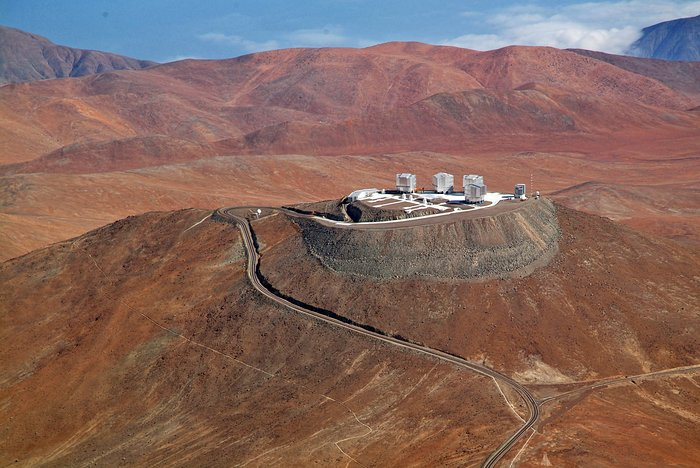
\includegraphics[width=0.7\textwidth]{Kap1/telescope.jpg}
\end{center}
\caption[short]{Vista aérea de la plataforma del ``ESO Very Large Telescope (VLT)", en la cima del Cerro Parnal, en el desierto chileno de Atacama. Créditos: J.L. Dauvergne  y G. Hüdepohl }
\label{fig:vvv_telescope}
\end{figure}

\par En este contexto, las estrellas variables de tipo RR Lyrae son una poderosa herramienta para obtener distancias a poblaciones de estrellas en la Vía Láctea, debido a que satisfacen una relación entre sus períodos y sus luminosidades absolutas que permite estimar distancias \cite{Shapley} \cite{Baade}. Sin embargo, a causa de la inmensa cantidad de información generada, la clasificación manual de estrellas se vuelve impracticable. Se requiere, por lo tanto, un método automatizado para identificar estrellas variables de tipo RR Lyrae de entre las $10^6-10^7$ estrellas variables que se espera encontrar en el área explorada \cite{jbc}. \\

\par Investigaciones recientes han mostrado que algoritmos de aprendizaje automatizado basados en ensambles de árboles tienen un excelente desempeño en este tipo de tareas, en tanto que otros métodos tradicionales como Support Vector Machines parecen no ser tan efectivos \cite{elorrieta} \cite{jbc}. El objetivo de esta tesina es intentar mejorar los resultados previos en el problema de detección de RR Lyrae en la VVV utilizando Support Vector Machines, así como comprender por qué métodos basados en ensambles de árboles aparentan funcionar mejor en este tipo de datos.  \\

\par Durante este trabajo se hizo uso de una amplia variedad de técnicas de aprendizaje automatizado, incluyendo diversos tipos de preprocesamiento, reducción de dimensionalidad y selección de variables, visualización de los datos y corrección de imbalance de clases. 

\section {Conceptos astronómicos}

\subsection{Estrellas RR Lyrae}

\par Una \textbf{estrella} es un objeto astronómico que consiste en una esfera luminosa de plasma, la cual mantiene su forma debido a su propia gravedad. Características como luminosidad, tamaño, evolución y duración de vida son definidas principalmente por su masa inicial. \\

\par Aquellas estrellas cuya luminosidad (magnitud aparente\footnote{Este valor indica la medida del brillo y cantidad de energía por segundo por metro cuadrado que se recibe de un objeto celeste por un observador en la Tierra. Como dicha cantidad recibida depende de la transmisión de la atmósfera en dichas bandas, las magnitudes aparentes se normalizan a un valor fuera de la atmósfera terrestre. La escala de magnitudes es una relación inversa logarítmica por la cual la estrella más brillante es la que tiene menor magnitud}) exhibe cambios periódicos o aleatorios se denominan \textbf{estrellas variables.} Las estrellas de tipo variable han jugado un rol crucial en la historia de la astronomía. El Catálogo General de Estrellas Variables \cite{catalogo} enumera más de 110 clases y subclases de estrellas variables. \\

\par Las estrellas variables pueden, en primera instancia, clasificarse en \textbf{variables intrínsecas} y \textbf{variables extrínsecas}, dependiendo del origen de la variabilidad observada. Si la causa de la variabilidad observada es inherente a la estrella, como es el caso de una estrella que periódicamente se expande y contrae, se le denomina intrínseca. Contrariamente, aquellas estrellas cuya variabilidad se debe a factores externos, como un compañero orbital que ocasionalmente la eclipsa, se denominan variables extrínsecas. \\

\par Probablemente el subgrupo más importante de las estrellas variables intrínsecas son las \textbf{estrellas pulsantes}, que varían en radio y luminosidad en el tiempo, expandiéndose y contrayéndose con períodos tan breves como minutos, o tan extensos como años, dependiendo del tamaño de la estrella. Para una revisión moderna de la fenomenología de estrellas pulsantes, puede remitirse a \cite{fisica}. \\

\par  Dentro de las estrellas pulsantes, se encuentran las subclases \textbf{RR Lyrae} y \textbf{Cepheids}, las cuales satisfacen una relación entre sus períodos y sus luminosidades absolutas que las convierte en invaluables herramientas para una de las tareas más complejas en astronomía: estimar distancias \cite{Shapley} \cite{Baade}. \\

\par Las estrellas de tipo \textbf{RR Lyrae} (en adelante, RRL) tienen períodos de entre 0.2 y 1.2 días \cite{smith}, y tienen una edad de aproximadamente 14 Gyr\footnote{1 gigayear (Gyr) = $10^9$ años}. Son consideradas excelentes candelas estándar, especialmente importantes a la hora de explorar distancias y propiedades de viejas problaciones estelares. Basándose en relevamientos recientes, se estima que hay alrededor de 140000 estrellas RRL en nuestra galaxia \cite{ogle} \cite{gaia} \\

\par En base a sus curvas de luz, las RRL fueron originalmente separadas en subtipos a, b y c \cite{bailey}, aunque posteriores trabajos unificaron los dos primeros subtipos en uno solo, RRab, dado que son fundamentalmente distintos del tercero, RRc \cite{schwarzschild}. Adicionales subtipos, extremadamente raros, fueron añadidos posteriormente. \\

\subsection{El relevamiento VVV}

\par ``Vista Variables in the Via Lactea (VVV) ESO Public Survey'' es un relevamiento fotométrico (terrestre) del bulbo galáctico y parte del disco interno de la Vía Láctea, que se llevó a cabo utilizando el telescopio VISTA en Parnal, Chile.  Uno de los objetivos principales de la VVV es adquirir un mayor entendimiento del origen, estructura y evolución de la Vía Láctea. Para una descripción detallada de la VVV puede consultarse \cite{vvv}, en tanto que un artículo más reciente con énfasis en variabilidad puede consultarse en \cite{vvv_actual} \\

\par El VVV, así como su sucesor el ``VVV Survey eXtended'', i.e. VVVX, persiguen el objetivo de producir un atlas profundo de una gran parte del Bulbo de la Vía Láctea, así como de una fracción del Disco Galáctico interno. Este mapa se produjo mediante un monitoreo sistemático de estas regiones, habiéndose completado 1929 horas de observación durante cinco años, comenzando en 2010. \\

\par Dentro del barrido total del relevamiento, es de interés astronómico la generación de catálogos de cualquier tipo de objeto, esperándose identificar no sólo estrellas variables, sino planetas, asteroides y otros fenómenos. En la figura \ref{fig:vvv_objects} se ilustra el número de fenómenos estimado.

\begin{figure}[h]
\begin{center}
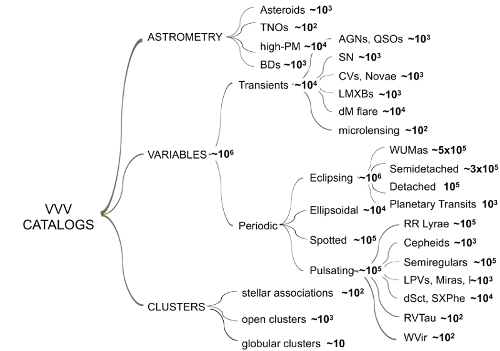
\includegraphics[width=0.7\textwidth]{Kap1/vvv_objects.png}
\end{center}
\caption[short]{Número esperado de fenómenos astrofísicos que espera detectar VVV en sus catálogos. Minniti et. al. 2010.}
\label{fig:vvv_objects}
\end{figure}

\par Los datos del VVV se presentan en una unidad llamada baldosa (tile, en inglés), una zona rectangular del cielo de $1.501 deg^2$ relevada a través del tiempo. Se requirieron 196 tiles para mapear el área del Bulbo, así como 152 tiles para el Disco. Cada tile se compone de varias imágenes en alta resolución para diferentes tipos de filtros (bandas anchas) de frecuencias lumínicas en el infrarrojo cercano (cinco en total). Asimismo, por cada imagen existe una base de datos con los valores de posición, magnitud y color de las fuentes de luz presentes en la imagen, llamada “catálogo fotométrico”. En el caso del VVV, la totalidad de las baldosas que constituyeron el relevamiento puede apreciarse en la figura \ref{fig:vvv_tiles} \\

\begin{figure}[h]
\begin{center}
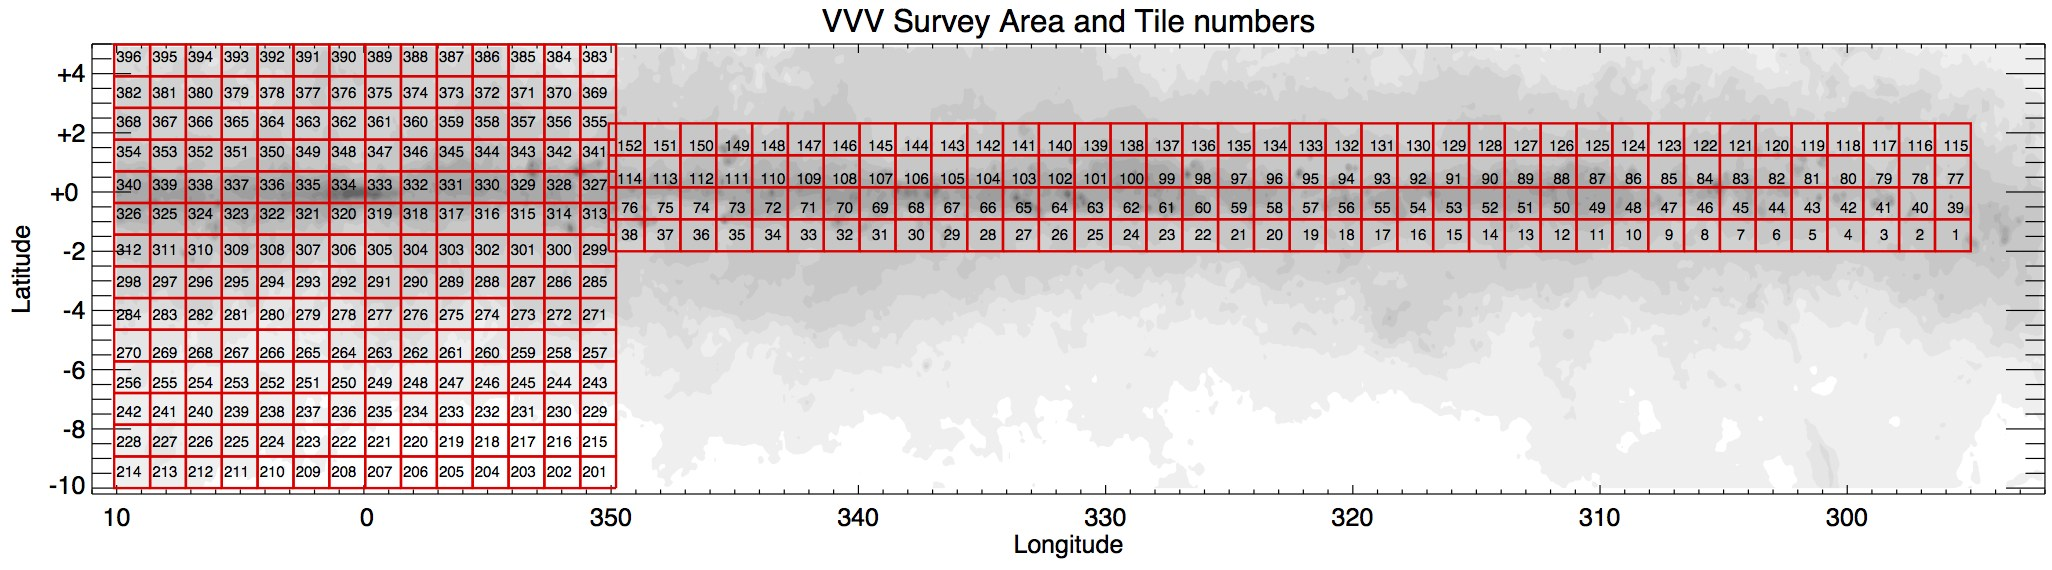
\includegraphics[width=\textwidth]{Kap1/vvv_tiles.jpg}
\end{center}
\caption[short]{Área del relevamiento VVV, en coordenadas galácticas. En escala de grises se puede apreciar la densidad estelar del área relevada. ~\protect\cite{Skrutskie_2006}}
\label{fig:vvv_tiles}
\end{figure}

\par La identificación de aquellas fuentes de luz que corresponden a estrellas RRL es de particular interés para VVV, dado que determinar distancias es vital para cumplir uno de sus objetivos primordiales: mapear el Bulbo Galáctico. Más aún, la existencia de trabajos previos \cite{gran1} \cite{gran2} que identifican algunos cientos de fuentes de luz como RRL dentro del área mapeada por la VVV, implica que se cuenta con un conjunto de datos que puede ser utilizado para entrenar y testear clasificadores de aprendizaje automatizado. 

\subsection{Extracción de atributos}

\par En esta tesina se hace un uso extensivo de los datos producidos en \cite{jbc}. Por cada tile en un subconjunto de tiles del relevamiento, se generó un dataset numérico, donde cada fila corresponde a una estrella, descripta por 62 atributos (del inglés, features) numéricas. En esta sección se explicará, a alto nivel, cómo se obtuvieron dichos atributos a partir de las mediciones de fotometría del infrarrojo cercano producidas por VVV. \\

\par Durante el relevamiento VVV se generaron enormes volúmenes de datos (1.4 TB/noche). El pipeline de VVV \cite{emerson} brinda, por cada imagen generada, una base de datos de archivos con los valores de posición, magnitud y color de las fuentes de luz presentes, llamada \textbf{catálogo fotométrico}. Aunque existen varios tipos de catálogos,  sólo dos son utilizados en este trabajo:

\begin{itemize}
\item En primer lugar, el catálogo \textbf{Pawprint Stack} contiene lecturas de los sensores infrarrojos de la cámara VIR-CAM del telescopio VISTA, correspondientes a la observación de un tile en una fecha dada (también llamado época). 
\item En segundo lugar, el catálogo \textbf{Band Merge} se utiliza para tener una lista confiable de estrellas en un cierto tile, dado que ciertas fuentes de luz pueden no estar presentes entre distintos Pawprint Stacks debido a condiciones meteorológicas o problemas en los instrumentos de medición.
\end{itemize}

\par Para determinar la variación en magnitud de cada estrella presente en cada Band Merge, fue necesario identificar todas sus ocurrencias en diferentes Pawprint Stacks. De esta forma, se puede formar una serie temporal de observaciones de la estrella en cuestión, haciendo uso de técnicas de cross-matching \cite{cross}. El resultado son series temporales como la que se puede apreciar en la figura \ref{fig:curva_de_luz}. Nótese que el tiempo de muestreo puede ser muy irregular, por lo que se presupone que es aleatorio. \\


\begin{figure}[h]
\begin{center}
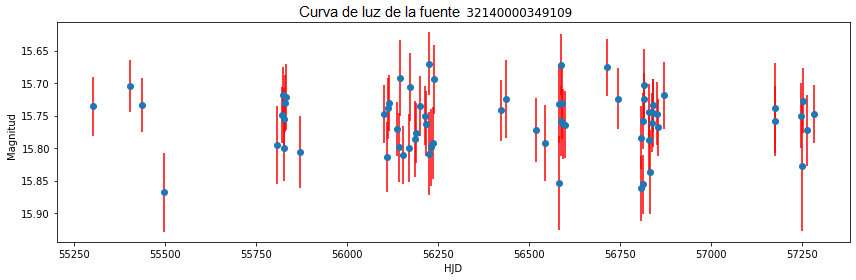
\includegraphics[width=\textwidth]{Kap1/light_curve.png}
\end{center}
\caption[short]{Curva de luz de una de las estrellas relevadas por VVV. El eje $x$ muestra el tiempo expresado en días heliocéntricos medios (HJD), en tanto que el eje $y$ muestra la magnitud aparente observada. Cada punto azul corresponde a una observación en un cierto Pawprint Stack, mientras que las líneas rojas indican el error asociado a cada medición. Imagen tomada de la documentación de Carpyncho, \url{https://carpyncho-py.readthedocs.io/} }
\label{fig:curva_de_luz}
\end{figure}

\par Habiéndose obtenido las series temporales de cada estrella, el siguiente paso fue estimar su período. Se utiliza el método de Fast Lomb-Scargle \cite{Lomb:1976wy} \cite{scargle} \cite{VanderPlas_2018} para recuperar cada período, el cual consiste en ajustar una función sinusoidal a los datos muestreados. \\

\par A partir de las curvas de luz y el período estimado, se extrajeron 49 atributos (o características) numéricas utilizando la herramienta \textit{Feets} \cite{cabral2018fats}. Estos atributos se refieren al período, variación de magnitud y morfología de las curvas de luz. Una descripción de cada atributo puede consultarse en el apéndice \ref{AnexoA}. \\

\par Una contribución original de \cite{jbc} fue la inclusión de atributos que describen las temperaturas o colores intrínsecos de cada estrella.  Dado que la presencia de polvo interestelar ocasiona un fenómeno denominado extinción, que provoca un enrojecimiento de los colores, fue necesario realizar una corrección utilizando mapas de extinción \cite{mcwilliam2011rr}. Como resultado final, se extrajeron 13 atributos numéricos describiendo el color de cada estrella. Nuevamente, la lista completa de atributos de color, junto con sus descripciones está disponible en el apéndice \ref{AnexoA}.

\subsection{Descripción de los datos}
\label{tiles_description}
En esta sección se describirán en detalle los datasets generados en \cite{jbc}, que pueden ser accedidos por el público a través de la librería Python \textbf{Carpyncho}\cite{carpynchoToolkit}.\\

Cada dataset generado corresponde a un cierto tile de la VVV. Cada fila de un dado dataset se corresponde a una cierta estrella variable, descripta por 62 atributos numéricos tal y como se describió en la sección anterior. La siguiente tabla resume los datos liberados por Carpyncho:

\begin{table}[h]
\centering
\begin{tabular}{|l|l|l|l|l|l|}
\hline
\textbf{Tile}  & \textbf{Épocas} & \textbf{Tamaño} & \textbf{RRL} & \textbf{Unknown} & \textbf{RRL / Tamaño} \\ \hline
b206           & 73              & 157825          & 47           & 157778           & 0.03\%                \\ \hline
b214           & 74              & 149557          & 34           & 149523           & 0.02\%                \\ \hline
b216           & 73              & 168996          & 43           & 168953           & 0.03\%                \\ \hline
b220           & 73              & 209798          & 65           & 209733           & 0.03\%                \\ \hline
b228           & 73              & 199853          & 28           & 199825           & 0.01\%                \\ \hline
b234           & 73              & 293013          & 126          & 292887           & 0.04\%                \\ \hline
b247           & 73              & 406386          & 192          & 406194           & 0.05\%                \\ \hline
b248           & 74              & 417839          & 218          & 417621           & 0.05\%                \\ \hline
b261           & 74              & 555693          & 252          & 555441           & 0.05\%                \\ \hline
b262           & 74              & 573873          & 314          & 573559           & 0.06\%                \\ \hline
b263           & 94              & 568110          & 317          & 567793           & 0.06\%                \\ \hline
b264           & 94              & 595234          & 307          & 594927           & 0.05\%                \\ \hline
b277           & 73              & 718567          & 429          & 718138           & 0.06\%                \\ \hline
b278           & 74              & 742153          & 436          & 741717           & 0.06\%                \\ \hline
b360           & 74              & 939110          & 669          & 938441           & 0.07\%                \\ \hline
b396           & 73              & 486639          & 15           & 486624           & 0.00\%                \\ \hline
\textbf{Total} & 1216            & 7182646         & 3492         & 7179154          & 0.05\%                \\ \hline
\end{tabular}
\end{table}

\par Como se puede observar, algunas de las estrellas variables de cada dataset están identificadas como RRL. Estas etiquetas provienen de realizar cross-matching con catálogos de estrellas variables de otros relevamientos con zonas de observación superpuestas a la VVV: \textit{OGLE-III} \cite{Udalski}, \textit{OGLE-IV} \cite{Udalski2} y VizieR \cite{vizier}. \\

\par En todos los experimentos de clasificación de este trabajo, se consideró como clase positiva a aquellas estrellas etiquetadas como RRL, siendo el resto la clase negativa. Es importante mencionar que nuestras clases positivas y negativas no son completamente certeras, dado que no han sido validadas con una inspección manual de cada fuente. Es posible que ciertas estrellas etiquetadas como RRL en realidad no lo sean y viceversa. Esto es especialmente válido en tiles como \textit{b396}, para las cuales hay pocas RRL previamente clasificadas en relevamientos anteriores. \\

\par Para la mayoría de los experimentos en este trabajo, se utilizó un subconjunto de tiles (\textit{b234}, \textit{b261}, \textit{b278} y \textit{b360} ) correspondiente a áreas del Bulbo que resultan de particular interés:

\begin{itemize}
\item Hay una buena densidad de RRL, pues las zonas se superponen bien con relevamientos anteriores. Por lo tanto, es probable que haya menos RRLs etiquetadas como no-RRL.

\item \textit{b278} es de particular interés pues contiene la llamada ventana de Baade, una zona con poco polvo intergaláctico en la línea visual de la tierra al núcleo galáctico \cite{Baade}. Esta zona ha sido históricamente utilizada para estudiar RRL.

\end{itemize}

\section {Aprendizaje automatizado}

Esta sección introducirá brevemente algunos conceptos básicos de aprendizaje automatizado, y está fuertemente basada en los capítulos introductorios de \cite{mitchell} y \cite{slearning}.

\subsection{Definición y tipos de aprendizaje}

El campo del \textbf{aprendizaje automatizado} consiste en el estudio de algoritmos que mejoran automáticamente su rendimiento gracias a la experiencia. Formalmente, Tom Mitchell en su libro \textit{ ``Machine Learning''} \cite{mitchell} define aprendizaje automatizado como sigue:

\begin{quotation}
Se dice que un programa de computadora aprende de la experiencia $E$ respecto a una tarea $T$ y una medida de desempeño $P$ , si el desempeño medido con $P$ en una tarea $T$ , mejora con la experiencia $E$.
\end{quotation}

Dada una muestra de datos, los algoritmos de aprendizaje automatizado construyen un modelo con el objeto de realizar predicciones o tomar decisiones \textit{sin haber sido expresamente programados para hacerlo}. Tales algoritmos pueden ser aplicados a un amplio rango de tareas, tales como aprender a conducir un vehículo autónomo \cite{Pomerleau-1989-15721}, aprender a jugar backgammon a nivel profesional \cite{Tesauro1995} o clasificar estructuras astronómicas \cite{clasify_astronomy}.  \\

Tradicionalmente, las distintas tareas a llevar a cabo por algoritmos de aprendizaje automatizado se dividen en tres paradigmas \cite{ai}:

\begin{itemize}
\item \textbf{Aprendizaje supervisado}: Consiste en aprender una función $f : I \mapsto O$, basándose en un conjunto de ejemplos $T \subset I \times O$ . En otras palabras, el algoritmo de aprendizaje automatizado intenta inferir una función a partir de un conjunto de entradas de ejemplo, etiquetadas con su valor de salida. Si el conjunto $O$ es discreto, se trata de una tarea de \textbf{clasificación}; en tanto que si es continuo, se trata de una tarea de \textbf{regresión}.
\item \textbf{Aprendizaje no supervisado}: En aprendizaje no supervisado, sólo hay entradas pero no salidas, por lo que el objetivo es aprender patrones y relaciones en conjuntos de datos no etiquetados.

\item \textbf{Aprendizaje por refuerzo (Reinforcement learning)}: Consiste en aprender a tomar decisiones en un ambiente dinámico, con el objeto de maximizar una cierta noción de recompensa acumulada. 
\end{itemize}

En este trabajo nos enfocaremos en técnicas de aprendizaje automatizado supervisado, dado que se desea abordar la tarea de clasificar estrellas variables en RRL o no-RRL. 

\subsection{Medidas de performance}
\label{ml_intro_test}
Como se mencionó anteriormente, el aprendizaje supervisado consiste en aproximar una función $f : I \mapsto O$. Durante una primera fase de \textbf{entrenamiento}, un conjunto de $n$ ejemplos $x_i \in I, \ i=1,\ldots,n$ junto con sus salidas asociadas $y_i \in O$ es utilizado para enseñar al modelo cómo estimar $f$. \\

Existe una amplia variedad de métodos de aprendizaje supervisado, y ninguno domina a todos los demás en todo conjunto de datos. El desempeño de cada método es altamente dependiente del problema a abordar, por lo que resulta de suma importancia decidir qué método produce los mejores resultados para un dado conjunto de datos. \\

Para evaluar el desempeño de un método, se necesita alguna forma de medir cuán bien el valor predicho por el método para una dada observación, se condice con la verdadera respuesta para esa observación. Sea $\hat{f}$ la estimación de $f$ obtenida por el método de aprendizaje supervisado en estudio:

\begin{itemize}

\item  En problemas de regresión, la métrica más comúnmente utilizada es el \textit{error cuadrático medio}:

\begin{center}
$MSE = \sum_{i=1}^{n} ( y_i - \hat{f}(x_i) )^2 $
\end{center}

\item En problemas de clasificación, podemos calcular la proporción de errores realizados:

\begin{center}
$Error \ Rate = \frac{1}{n} \sum_{i=1}^{n} I( y_i , \hat{f}(x_i) ) $
\end{center}

Donde:
\begin{center}
$
I(y_i,\hat{y_i}) =
\left\{
	\begin{array}{ll}
		0  & \mbox{si } y_i = \hat{y_i} \\
		1 & \mbox{si } y_i \neq \hat{y_i}
	\end{array}
\right.
$
\end{center}

\end{itemize}

Ambas métricas fueron definidas sobre los datos de entrenamiento. Sin embargo, en general, no nos importa cuán bien el método funciona en los datos de entrenamiento. Estamos interesados en las métricas obtenidas al aplicar nuestro modelo ya entrenado a un conjunto de datos de test, que no hayan sido previamente utilizados en la fase de entrenamiento. \\

Esto nos lleva a la distinción entre \textit{training MSE} y \textit{training Error Rate}, en contraposición a \textit{test MSE} y \textit{test Error Rate}. Usualmente, se reserva una porción de los datos disponibles para ser utilizada como \textbf{conjunto de test}. Estos datos no son utilizados en la fase de entrenamiento, y son utilizados para calcular métricas como \textit{test Error Rate} una vez terminada la fase de entrenamiento. Tales métricas proveen una noción de cuán bien el clasificador funcionará en datos no antes vistos. Una alternativa para obtener tales métricas sin necesidad de tener un conjunto separado de test es utilizar \textbf{cross validation} \cite{cross_validation}. \\

En este trabajo estamos particularmente interesados en problemas de \textbf{clasificación binaria}, es decir, problemas de aprendizaje automatizado supervisado en los cuales el conjunto de etiquetas contiene solo dos elementos, o clases, a menudo llamados clase positiva y negativa. En problemas de clasificación binaria, cada elemento se puede clasificar en una de las siguientes cuatro categorías: \\

\begin{table}[h!]
\begin{tabular}{l|l|l|}
\cline{2-3}
                                                    & \textbf{Clase predicha: Negativa} & \textbf{Clase predicha: Positiva} \\ \hline
\multicolumn{1}{|l|}{\textbf{Clase real: Negativa}} & Verdadero negativo (TN)           & Falso positivo (FP)               \\ \hline
\multicolumn{1}{|l|}{\textbf{Clase real: Positiva}} & Falso negativo (FN)               & Verdadero positivo (TP)           \\ \hline
\end{tabular}
\end{table}

Los falsos positivos son aquellos elementos de clase negativa, clasificados incorrectamente con etiqueta positiva. Similarmente, los falsos negativos son aquellos elementos con etiqueta positiva, clasificados como negativos. Los verdaderos positivos (negativos), son aquellos elementos positivos (negativos), que fueron clasificados correctamente. \\

Dado un cierto conjunto de datos etiquetados, la performance de un clasificador binario puede visualizarse al calcular una \textbf{matriz de confusión}. La matriz de confusión mostrará la suma de elementos de cada una de las cuatro categorías explicadas. En particular, podemos reescribir la métrica Error Rate como: \\

\begin{center}
$ Error Rate = \frac{FP + FN}{FP + FN + TP + TN} $
\end{center}

Equivalentemente, es usual analizar la \textbf{tasa de aciertos}:

\begin{center}
$ Acc = \frac{TP + TN}{FP + FN + TP + TN} $
\end{center}

\subsection{Problemas desbalanceados}
\label{imbalance}

A la hora de estudiar problemas de clasificación, es importante tener en cuenta la proporción de datos de cada clase. Un \textbf{problema de clasificación desbalanceado} es aquel en el cual la cantidad de elementos de cada clase no es proporcional. Ciertas aplicaciones como diagnóstico médico o detección de transacciones fraudulentas con tarjeta de crédito presentan datasets con un número muy pequeño de instancias positivas\footnote{En problemas de clasificación binaria, usualmente se considera clase positiva a la clase minoritaria, en tanto que la clase mayoritaria es la negativa}, que son sin embargo cruciales de clasificar correctamente \cite{imbalanced_svm}. \\

Si se utilizan datasets imbalanceados para entrenar y testear, es inadecuado utilizar métricas de desempeño basadas en clasificar la \textit{mayor cantidad} de elementos de forma correcta, como $Acc$. La hipótesis mas sencilla, clasificar todas las instancias como pertenecientes a la clase mayoritaria, a menudo maximiza tales métricas. \\

Un primer paso a la hora de trabajar con datos desbalanceados es, entonces, utilizar métricas que no son sensitivas al imbalance de clases. En clasificación binaria, las siguientes métricas son de interés:

\begin{itemize}
\item \textbf{Precisión}: La proporción de instancias clasificadas como positivas, que realmente lo son:
\begin{center}
$ Precision =  \frac{TP}{TP + FP}$
\end{center}

\item \textbf{Recall}: La proporción de instancias positivas que son detectadas por el clasificador.
\begin{center}
$ Recall =  \frac{TP}{TP + FN}$
\end{center}

\end{itemize}

A menudo, muchos métodos de aprendizaje automatizado para clasificación binaria producen un puntaje\footnote{Se utiliza el término puntaje (del inglés \textit{score}), dado que no se utilizará un enfoque probabilístico.} en $[0,1]$ para cada instancia a clasificar. Puntajes cercanos a 0 indican que el clasificador tiene mayor certeza de que una cierta entrada pertenece a la clase negativa, en tanto que valores cercanos a 1 indican pertenencia a la clase positiva. \\

En tal escenario, resulta necesaria la elección de un umbral $t \in [0,1]$, de forma tal que sólo instancias cuyos puntajes son mayores a $t$ sean clasificadas como positivas, siendo las demás negativas. En consecuencia, resulta importante determinar un $t$ adecuado para el dominio de aplicación en estudio, dado que distintos valores de $t$ tendrán un impacto directo en la matriz de confusión producida. \\

Valores altos de $t$ tenderán a producir clasificadores con mayor precisión y menor recall, en tanto que valores pequeños de $t$ tenderán a clasificadores con mayor recall y menor precisión. Una forma gráfica de analizar esta correspondencia es a través de la curva de precision-recall del clasificador, como la de la figura \ref{fig:prc}, en la cuál se grafica la precisión y el recall obtenidos para un rango de valores de $t$. \\

\begin{figure}[h]
\begin{center}
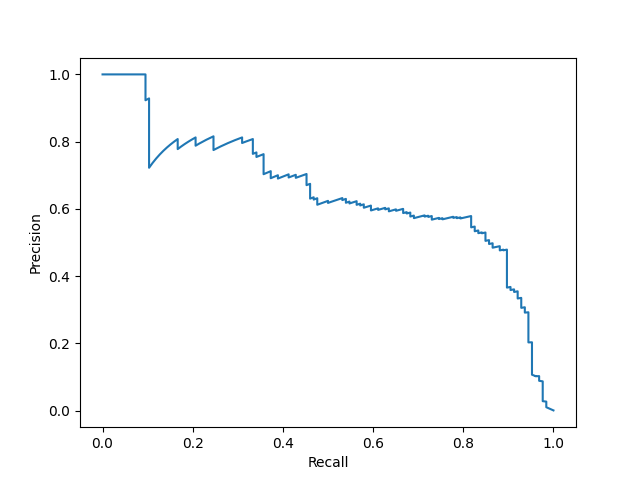
\includegraphics[width=.6\textwidth]{Kap1/PRc.png}
\end{center}
\caption[short]{Ejemplo de una curva de precision-recall. Cada punto de la curva corresponde a la precisión y el recall obtenidos para un cierto valor de $t$. }
\label{fig:prc}
\end{figure}

Si se está abordando un problema desbalanceado, una forma determinar si un clasificador tiene mejor performance que otro es comparar sus curvas de precision-recall en el dataset de test. Dado que las curvas de precision-recall tienden a ser bastante ruidosas en áreas de bajo recall, en este trabajo se utilizó en repetidas ocasiones el área bajo la curva de precision-recall restringida al dominio [0.35,1] para obtener una medida de performance numérica, a la que llamaremos R-AUPRC (del inglés Robust Area Under the Precision Recall Curve, área debajo de la curva de precision-recall robusta).\\


R-AUPRC resulta útil cuando se desea comparar decenas o cientos de curvas a la vez, siendo imposible su inspección visual y prefiriéndose aquel modelo que maximiza el R-AUPRC. Otra métrica alternativa es utilizar la precisión del clasificador a un cierto valor fijo de recall. \\

Además de utilizar métricas adecuadas para evaluar el desempeño, otras técnicas para trabajar con datos desbalanceados son:

\begin{itemize}
\item Corregir manualmente el imbalance de clases en los datos. Una posibilidad es eliminar datos de la clase mayoritaria aleatoriamente (\textbf{undersampling}) \cite{nathalie} hasta alcanzar el balance deseado. Una segunda posibilidad es generar nuevas instancias de la clase minoritaria (\textbf{oversampling}). \cite{he}
\item Forzar a que el clasificador preste más atención a la clase minoritaria \cite{imbalanced_svm}. Por ejemplo, como se verá en secciones posteriores, para ciertos métodos de aprendizaje automatizado como Support Vector Machines es posible asociar un peso (\textit{class\_weight}) a cada clase, de tal forma que el clasificador será menos permisivo a la hora de clasificar incorrectamente clases con alto peso.
\end{itemize}

\subsection{Árboles de decisión}
En esta sección se presentará brevemente uno de los métodos de aprendizaje automatizado supervisado para clasificación más ampliamente utilizado: Árboles de Decisión\cite{mitchell}. \\

Los árboles de decisión están formados por dos tipos de elementos: nodos y ramas. En primer lugar, veamos cómo se usa un árbol de decisión ya construido. En la figura \ref{fig:tree} podemos ver un ejemplo de un árbol de decisión que intenta predecir si un pasajero sobreviviría o no al hundimiento del Titanic.  \\

Supongamos que cada persona está descripta por tres atributos numéricos: edad, género y número de familiares en el barco (sibsp). Para clasificar una nueva instancia, se desciende por el árbol comenzando por la raíz. En cada nodo, se realiza una comparación sobre un atributo de la instancia a clasificar, y se desciende por una de las dos ramas del árbol de acuerdo al resultado. \\

\begin{figure}[h!]
\begin{center}
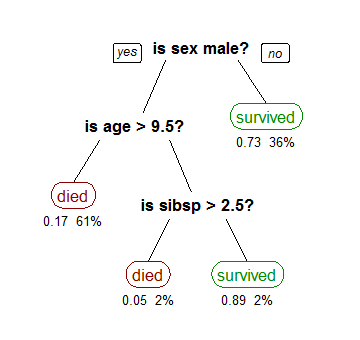
\includegraphics[width=.44\textwidth]{Kap1/tree.png}
\end{center}
\caption[short]{Árbol de decisión construido sobre el dataset \textit{Titanic}. Los árboles de decisión se dibujan invertidos, con la raíz en la parte superior. Créditos: Wikipedia. }
\label{fig:tree}
\end{figure}

El proceso continúa hasta llegar a un nodo que no posee más subdivisiones, tales nodos son llamados \textbf{hojas} e indicarán la clase final que con la cual el clasificador etiquetará la nueva instancia. \\

Ahora que ya se ha discutido cómo utilizar un árbol de decisión existente, veamos cómo se crea un nuevo árbol a partir de un conjunto de entrenamiento. Un algoritmo greedy para crecer un árbol de decisión consiste en crear cada nodo recursivamente, comenzando desde la raíz. Naturalmente, se debe decidir qué atributo utilizar en cada nodo no hoja para realizar la división; así como el valor de corte que se utilizará (\textit{split} en inglés). A la hora de crear un nodo, se considerará para cada atributo un cierto número de valores de corte, y se elegirá aquel que minimice una cierta métrica de costo sobre los datos de entrenamiento. \\

Distintas métricas pueden utilizarse para decidir cuál es el mejor split, intentando incentivar la homogeneidad de la variable objetivo en los subconjuntos producidos. Dos métricas muy populares son \textit{Gini Impurity} e \textit{Information Gain} \cite{ginigain}.\\

Un aspecto a considerar es cuándo detener este proceso de crecimiento. Es posible que árboles extremadamente complejos conduzcan a \textbf{sobreajuste} (overfitting en inglés), un fenómeno en el cual un método de aprendizaje automatizado se ajusta demasiado bien a los datos de entrenamiento, aprendiendo detalles y ruido presentes; y por lo tanto perdiendo desempeño al clasificar instancias nuevas. Por lo tanto, puede ser valioso detener el crecimiento del árbol prematuramente.%, o bien \textit{podarlo} (eliminar algunos nodos) posteriormente. 

\subsection{Random Forests}

En esta sección se introducirá brevemente uno de los dos métodos de clasificación utilizados en este trabajo: Random Forests \cite{rf}. Random Forest es un método \textbf{ensamble}, más específicamente de tipo \textbf{bagging}. \\

Los métodos ensamble consisten en utilizar \textit{múltiples} algoritmos de aprendizaje para mejorar el desempeño que cada uno de ellos tiene individualmente. En concreto, los métodos de bagging \cite{bagging} se basan en generar múltiples versiones de un mismo predictor, perturbando los datos de entrenamiento que se le suministran a cada uno, y combinando sus resultados para formar un clasificador más potente. \\

En particular, Random Forest es un ensamble donde los predictores individuales son árboles de decisión. Un Random Forest formado por $n$ árboles de decisión, se construye de la siguiente forma:

\begin{enumerate}
\item \textbf{Crear un bootstrap del dataset de entrenamiento por cada árbol a construir}: En lugar de utilizar el dataset de entrenamiento completo para entrenar cada árbol de decisión, se calculará un bootstrap (sampleo aleatorio con reemplazo) por cada árbol de decisión a entrenar. 
\item \textbf{Entrenar cada árbol de decisión}: Se entrena cada árbol de decisión utilizando uno de los bootstraps generados en el paso anterior. Para añadir aún más aleatoriedad, se considera únicamente un subconjunto aleatorio de atributos en cada nodo a la hora de elegir el mejor split.
\end{enumerate}

Una de las principales desventajas de los árboles de decisión es que tienen tendencia a sobreajustar los datos de entrenamiento. La aleatoriedad involucrada en el primer paso, implica que si bien cada árbol puede sobreajustar sus datos de entrenamiento; el Random Forest completo no sobreajustará ningún subconjunto de datos en especial. \\

Los métodos ensamble funcionan mejor si hay una cierta decorrelación, o variedad, en los modelos individuales. La aleatoriedad involucrada en el segundo paso también contribuye a esta decorrelación, evitando que ciertos atributos con alto poder predictivo sean incluidos en todos los árboles. \\

Una vez que el random forest ha sido construido, realizar predicciones para nuevas instancias es muy sencillo. Se evalúa la entrada en cuestión en cada uno de los árboles, obteniendo $n$ predicciones que se combinan para formar la predicción final del random forest. En problemas de clasificación, cada predicción puede considerarse un voto, y la predicción más votada será la predicción del random forest.\\

Random Forest es un método muy flexible y poderoso, y es cotidianamente utilizado en aplicaciones industriales. Una de sus principales ventajas es su facilidad de uso, dado que no se requiere la optimización de hiperparámetros complejos y brinda generalmente buenos resultados.

\subsection{Support Vector Machines}

\label{trick}

En esta sección se presentará el segundo método de aprendizaje automatizado supervisado para clasificación binaria que se utilizará en este trabajo: Support Vector Machines (SVM) \cite{svm2} \cite{svm}  \\

Una tarea de clasificación binaria puede ser vista como la tarea de separar las clases en el espacio de atributos. En la figura \ref{fig:sv1} podemos ver un ejemplo en el cual se decide utilizar un hiperplano para realizar dicha separación. Como se puede ver hay infinitos separadores lineales para este ejemplo. \\

\begin{figure}[h!]
\begin{center}
  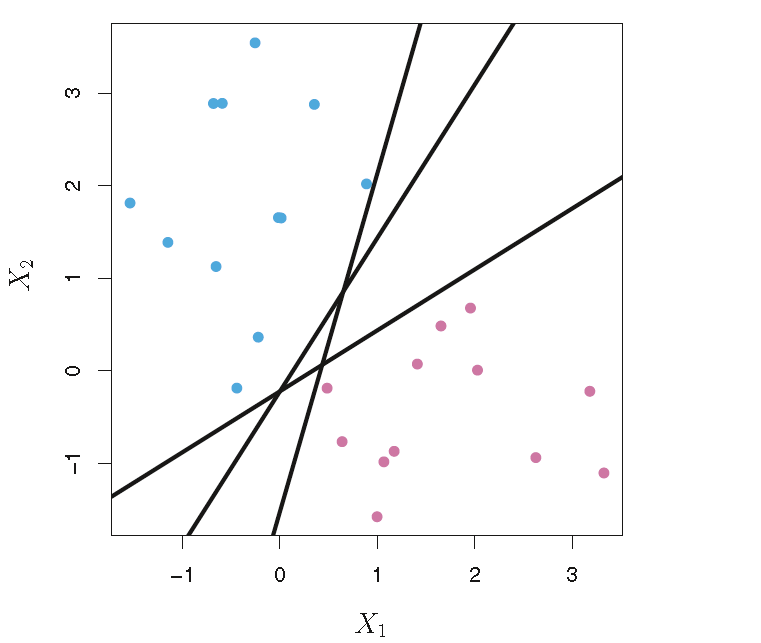
\includegraphics[width=0.56\textwidth]{Kap1/svm1.png} 
\end{center}
\caption{ En esta imagen podemos ver un ejemplo de clasificación binaria utilizando un separador lineal. Se ilustra la existencia de múltiples separadores lineales que podrían ser utilizados. Créditos: Drew Wilimitis, \url{towardsdatascience.com}.}
\label{fig:sv1}
\end{figure}

Las SVM buscan elegir el hiperplano que separe ambas clases maximizando el margen entre ambas clases, donde el margen se define como la mínima distancia entre un punto de training y el hiperplano separador. Esta situación se ilustra en la figura \ref{fig:svm_3}. \\

\begin{figure}[h!]
\begin{center}
  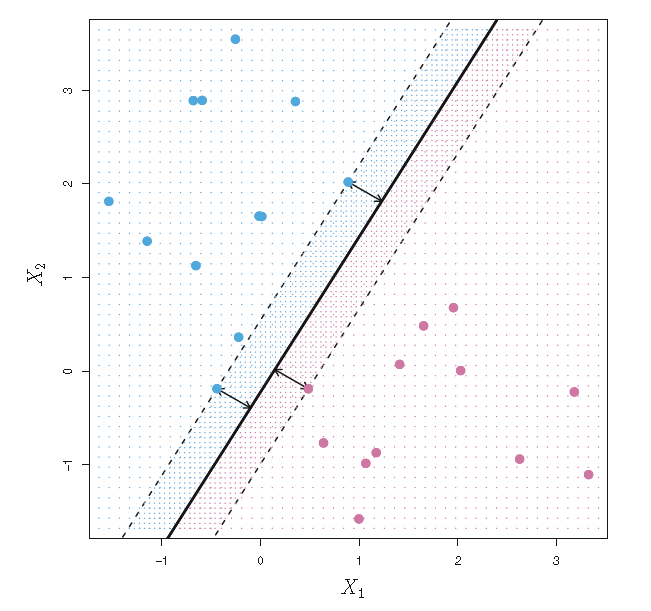
\includegraphics[width=0.56\textwidth]{Kap1/svm3.png} 
  \end{center}
 \caption{En esta imagen se ilustra el hiperplano escogido por SVM. Aquellos puntos que están a la menor distancia del hiperplano separador se denominan vectores soporte. SVM escoge el hiperplano que maximiza la separación entre ambas clases. Créditos: Drew Wilimitis, \url{towardsdatascience.com}}
\label{fig:svm_3}
\end{figure}


Un problema inmediato a considerar es que la frontera que separa las clases puede estar determinada por una superficie no lineal. Esto puede solucionarse mediante el uso de una función kernel, que mapea los datos a algún espacio de mayor dimensionalidad donde la frontera que separa las clases será, potencialmente, lineal. Esta situación es ilustrada en la figura \ref{fig:svm_4}\\

\begin{figure}[h!]
\begin{center}
  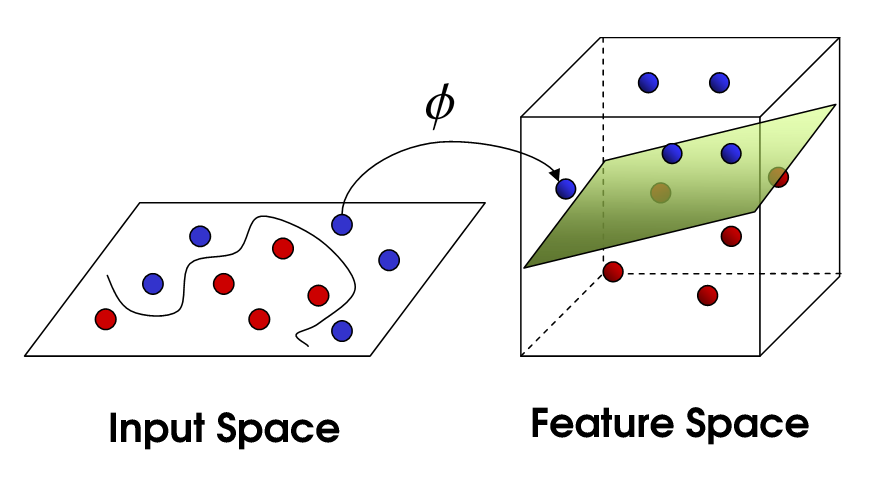
\includegraphics[width=0.7\textwidth]{Kap1/svm5.png} 
  \end{center}
 \caption{ Utilización de una función kernel para mapear puntos que no son linealmente separables a un espacio de mayor dimensionalidad, donde pueden ser separados por un hiperplano. Créditos: Drew Wilimitis, \url{towardsdatascience.com} }
\label{fig:svm_4}
\end{figure}

Matemáticamente, dado un conjunto de entrenamiento $\{ (x_i,y_i), \ i=1 \ldots l, \ x_i \in R^n \ , y_i \in \{1,-1\} \}$, SVM requiere solucionar el siguiente problema de optimización:

\begin{center}
$\begin{aligned}
\min_{w,b,\xi} \quad & \frac{1}{2}w^{t}w+C\sum_{i=1}^{l}{\xi_{i}}\\
\textrm{s.t.} \quad & y_{i}(w^T\phi(x_{i})+b) \geq 1 - \xi_{i}\\
  &\xi\geq0    \\
\end{aligned}
$
\end{center}

Nótese que los vectores de entrenamiento $x_i$ son mapeados a un espacio de mayor dimensionalidad (quizás infinita) a través de la función $\phi$. SVM encuentra un hiperplano que separa ambas clases con el máximo margen posible. \\

$C>0$ es un hiperparámetro de penalidad que regula cuánto error se permite, introduciendo  variables slack $\xi_i$ que permiten a algunos vectores estar del lado equivocado de la frontera. Esta situación es ilustrada en la figura \ref{fig:svm_5}\\


\begin{figure}[h!]
\begin{center}
  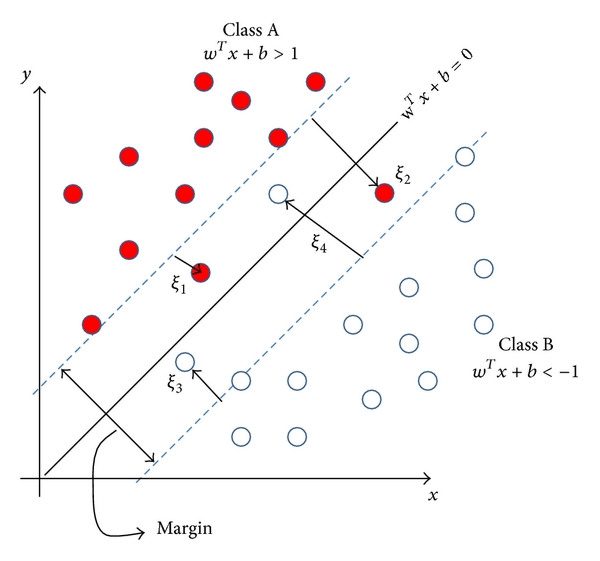
\includegraphics[width=0.4\textwidth]{Kap1/slack.jpg} 
  \end{center}
 \caption{ Utilización de variables slack que permiten a algunos puntos de entrenamiento estar dentro del margen, e incluso del lado equivocado del hiperplano. El parámetro C permite regular cuán permisivo es el modelo a la hora de permitir errores de clasificación. Imagen tomada de \textit{Hybrid Model Based on Genetic Algorithms and SVM Applied to Variable Selection within Fruit Juice Classification}, Carlos Fernandez-Lozano et al. }
\label{fig:svm_5}
\end{figure}

$K(x_i,x_j) = \phi(x_i)^T \phi(x_j)$ es llamada \textbf{función kernel}. Algunas de las funciones kernel más populares son:

\begin{itemize}
\item \textbf{Lineal}: $K(x_i,x_j) = x_i^T x_j$
\item \textbf{Polinomial}: $K(x_i,x_j)= (\gamma x_i^T x_j + r)^d , \ \gamma > 0$
\item \textbf{Radial Basis Function (RBF)}: $K(x_i,x_j)= exp (-\gamma\left\| x_i - x_j \right\|^2  ), \ \gamma>0.$

\end{itemize}

Donde $\gamma$ y $d$ son parámetros del kernel. Una vez que se han escogido los hiperparámetros necesarios, y se ha hallado el hiperplano separador óptimo, es muy sencillo realizar predicciones para nuevas instancias: se asignará una clase de acuerdo al lado del hiperplano separador en que la nueva instancia se encuentra.  \\

SVM es uno de los métodos de predicción con mayor sustento teórico, dado que se basa en aprendizaje estadístico o teoría VC (Vapnik-Chervonenkis). \cite{vapnik71uniform} \cite{vapnik74theory}.

\subsection{El dilema sesgo-varianza}

En esta sección, se discutirá brevemente el dilema sesgo-varianza en aprendizaje automatizado \cite{statisticallearning}. Supongamos que la variable que estamos intentando predecir es $Y$, basándonos en un conjunto de atributos $X$. Asumimos que hay una relación subyacente entre ambos:
\begin{center}
$Y = f(X) + \epsilon$
\end{center}

Donde $\epsilon$ se distribuye de forma normal, con media cero y varianza $\sigma^2$. Utilizando algún algoritmo de aprendizaje automatizado, y a partir de un dataset de entrenamiento $D$, se obtiene un modelo $\bar{f}$ que intenta aproximar $f$. El error cuadrático de predicción para un input $x$ es:\\

\begin{center}
$Err(x) = E[(Y-\bar{f}(x))^2]$
\end{center}

Lo cual puede reescribirse como:

\begin{center}
$Err(x) = (E[\bar{f}(x)]-f(x))^2 + E[(\bar{f}(x)-E[\bar{f}(x)])^2] + \sigma^2$ 
\end{center}

Donde podemos darle un nombre a cada término de esa suma:

\begin{center}
$Err(x) =  Sesgo^2 + Varianza + Error Irreducible$
\end{center}

Nótese que las esperanzas se calculan sobre las diferentes elecciones de dataset de entrenamiento $D$. \\

El \textbf{error irreducible}, que es la varianza de la función objetivo, está fuera de nuestro control. No puede ser reducido creando buenos modelos, y es una medida de la cantidad de ruido en nuestros datos. Los otros dos términos, en cambio, están bajo nuestro control.\\

El \textbf{sesgo} es la diferencia entre la predicción promedio de nuestro modelo, y el valor correcto que intentamos predecir. Este error puede ser pensado como el error causado por asunciones simplistas del modelo, como por ejemplo asumir que la distribución de los datos es lineal. Un modelo con alto sesgo presta muy poca atención a los datos de entrenamiento. \\

La \textbf{varianza} es la variabilidad de la predicción de un modelo, es decir, cuánto varía $\bar{f}(x)$ alrededor de su media. Modelos con alta varianza prestan mucha atención a los datos de entrenamiento, pero no generalizan tan bien en datos no vistos anteriormente. \\

De forma general, cuando la complejidad de nuestro modelo crece, la varianza tiende a aumentar en tanto que el sesgo disminuye. Lo opuesto sucede cuando la complejidad del modelo disminuye. \\

La figura \ref{fig:tradeoff} muestra el comportamiento típico de la varianza y el sesgo en función de la complejidad del modelo. El error de entrenamiento tiende a decrecer cuando incrementamos la complejidad del modelo, es decir, cuando ajustamos los datos con mayor precisión. Sin embargo, un exceso de ajuste (\textbf{overfitting}) conduce a un modelo que se adapta demasiado a los datos de entrenamientos, y no generaliza bien en test. En este caso, las predicciones tendrán gran varianza. En contraste, si el modelo no es muy complejo, no se ajusta lo suficiente a los datos de entrenamiento (\textbf{underfitting}) y tendrá un alto sesgo, resultando nuevamente en alto error de generalización.\\ 

\begin{figure}[h!]
\begin{center}
  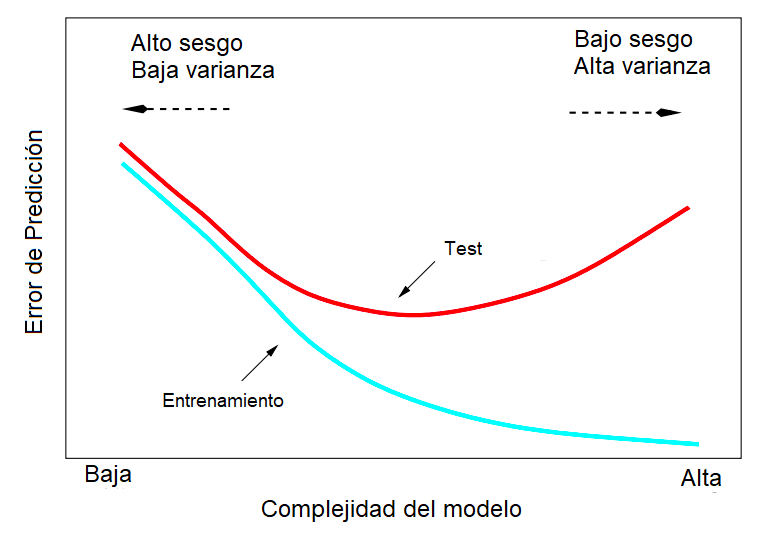
\includegraphics[width=0.7\textwidth]{Kap1/tradeoff.png} 
  \end{center}
 \caption{ Error de test y de entrenamiento en función de la complejidad del modelo. Créditos: \protect\cite{statisticallearning} }
\label{fig:tradeoff}
\end{figure}

\section{Antecedentes relevantes a esta tesina}

\par Como se adelantó anteriormente, en esta tesina se estudiará la aplicación de algoritmos de aprendizaje automatizado al problema de clasificar estrellas variables de tipo RRL en los datasets publicados por Carpyncho, correspondientes al relevamiento VVV. \\

\par Previamente, se ha explorado el desempeño de clasificadores automatizados de estrellas variables en varios estudios \cite{ej1}, \cite{ej2}, \cite{ej3}, \cite{ej4}.  Los dos antecedentes más relevantes de esta tesina, \cite{elorrieta} y \cite{jbc}, proponen procedimientos automatizados para clasificar RRL de subtipo ab en la VVV, basándose en sus curvas de luz. \\

En \cite{elorrieta} se concluye que AdaBoost\cite{adaboost}, un método basado en ensambles de árboles, obtiene consistentemente el mejor desempeño de entre una amplia selección de algoritmos de aprendizaje automatizado incluyendo SVM y redes neuronales profundas. El desempeño es estimado utilizando cross-validation, y a través de la comparación entre dos datasets que fueron clasificados por expertos humanos. Nótese que varias de las métricas utilizadas en este trabajo, como AUC o $F_1$, no son adecuadas para trabajar con datasets altamente desbalanceados. \\

Posteriormente, en \cite{jbc}, se refinaron las métricas de desempeño y se extiende el conjunto de atributos utilizado para describir estrellas variables, incorporando atributos de pseudocolor. En uno de los experimentos, se realizó una comparación entre el desempeño de distintos métodos de clasificación, incluyendo Random Forests y SVM. El mayor desempeño se obtuvo, nuevamente, utilizando ensambles de árboles.


\section{ Comparación entre Random Forest y Support Vector Machines}

Como ya se ha mencionado, Random Forest y SVM son dos potentes métodos de aprendizaje automatizado, que pueden ser aplicados tanto a problemas de regresión como de clasificación. En esta sección, se hará hincapié en ciertas características que distinguen ambos métodos, buscando comparar y contrastar la forma en que ambos operan. El objetivo es enumerar razones que puedan explicar por qué Random Forest parece funcionar mejor que SVM en estudios previos de clasificación de RRL.\\

En primer lugar, se debe notar que ambos métodos proceden de formas radicalmente distintas. En la fase de training, los árboles de decisión que conforman un random forest observan cada atributo uno a la vez, analizando si es beneficioso realizar divisiones para ciertos valores \cite{mitchell}. Por otro lado, las SVM consideran cada elemento del dataset como un punto en el espacio, utilizando los valores de todos los atributos en simultáneo para calcular un hiperplano separador \cite{svm2}. \\

Una primera consecuencia es que RF es inmune a \textbf{diferentes escalas} en los atributos \cite{statisticallearning}. Los datos no necesitan estar normalizados ni centrados para que RF funcione, mientras que la naturaleza geométrica de SVM implica que los distintos atributos necesariamente han de estar expresados en la misma escala \cite{svm_practical}. Más aún, las rutinas de optimización que usualmente implementan la fase de training en SVM pueden fallar en converger, o tardar significativamente más tiempo, si los datos no se encuentran escalados a [0,1] o [-1,1]
\cite{svm_practical}. Por lo tanto, resulta vital realizar un preprocesamiento adecuado a los datos a la hora de aplicar SVM. \\ 

Una segunda consecuencia es que RF puede \textbf{ignorar atrobitps que no son muy informativos} fácilmente, pues los árboles de decisión tienen un mecanismo simple para darse cuenta de que no sirven (ningún split será un buen candidato) \cite{statisticallearning}. De acuerdo a \cite{statisticallearning}, los árboles de decisión ``realizan una selección de variables internamente como una parte integral en su forma de proceder''. Ignorar atributos no informativos puede ser más complejo para SVM, pues la rutina de optimización tendrá que asignar un valor nulo a los coeficientes correspondientes en $w$. Un cierto atributo puede ser poco informativo por distintos motivos: puede haber sido incluido en el dataset pero no contener información relevante para predecir la variable target, puede ser extremadamente ruidoso, etc.  Las técnicas de selección de variables  (Feature Selection) que se aplicarán en capítulos posteriores son una forma adecuada de deshacerse de atributos no informativos, y deberían reducir el impacto de este problema en SVM. \\

Una tercera consecuencia es que RF no se ve afectado por \textbf{atributos altamente correlacionados}, pues cada árbol de decisión se dará cuenta fácilmente de que no es informativo realizar el mismo split en dos atributos correlacionados \cite{rf_collinearity}. Por otro lado, puede ser más complejo para SVM aprender a ponderar correctamente información redundante. Por tal motivo, es interesante explorar correlaciones entre atributos y analizar el impacto de eliminar redundancias en los datos. \\

Otro punto a considerar es cómo manejar el \textbf{overfitting} (sobreajuste) durante la fase de training. SVM requiere una cuidadosa estimación del hiperparámetro de regularización C para controlar este fenómeno, mientras que Random Forest por su naturaleza de ensamble es inmune a sobreajustar al aumentar el número de árboles \cite{rf}. Más aún, si se utiliza un kernel con parámetros adicionales como RBF en SVM, se requiere estimar cuidadosamente otros \textbf{hiperparámetros}, por ejemplo realizando Cross Validation Grid Search \cite{svm_practical}. Contrariamente, Random Forest es considerado un método off-the-shelf \cite{offshelf}, pues suele producir buenos resultados sin una optimización de hiperparámetros meticulosa. Por lo tanto, resulta de vital importancia una cuidadosa optimización de hiperparámetros de regularización y de kernel en SVM. \\

El marcado \textbf{imbalance de clases} presente en los datos, con aproximadamente 2000 elementos de clase negativa (no-RRL) por cada elemento de clase positiva (RRL), puede afectar negativamente el desempeño de RF y SVM. En \cite{jbc}, se determinó que corregir el imbalance de clases de estos datos mediante undersampling conduce a una pérdida de desempeño en Random Forest, siendo conveniente entrenar los modelos utilizando los datos sin balancear. Por otro lado, es posible que esto no sea cierto para SVM, dado que el imbalance de clases puede ocasionar pérdida de performance pues el hiperplano soporte elegido estará más alejado de la clase positiva, y habrá mayor cantidad de vectores soporte de la clase negativa \cite{imbalanced_svm}. Resulta por lo tanto interesante explorar diversas técnicas de undersampling y oversampling a la hora de aplicar SVM. \\

La existencia de \textbf{atributos ruidosos y outliers} en los datos es de esperarse en datasets astronómicos, que pueden incluir errores de medición y observación. RF no se ve afectado por outliers, pues los árboles de decisión funcionan creando cubetas (bins) que no se ven influenciadas por valores extremos \cite{statisticallearning}. Atributos que son altamente ruidosos no serán informativos a la hora de dividir la clase objetivo, y podrán ser ignorados por los árboles de decisión. Es interesante explorar distintos preprocesamientos tendientes a limpiar o suavizar los datos a la hora de aplicar SVM, pues puede ayudar a mitigar el efecto de outliers y ruido en los datos. \\

La siguiente tabla resume los puntos discutidos en esta sección. Durante el resto de este trabajo, se explorará cada uno de ellos. 

\begin{table}[h!]
\begin{tabular}{|l|l|}
\hline
\textbf{Aspecto}                                                                            & \textbf{Capítulo Relevante}                                  \\ \hline
\begin{tabular}[c]{@{}l@{}}Estimación de hiperparámetros óptimos\\ Overfitting\end{tabular} & Capítulos 2, 3.                                              \\ \hline
Diferentes escalas en los datos                                                             & Capítulo 4: Preprocesamientos                                \\ \hline
\begin{tabular}[c]{@{}l@{}}Atributos ruidosos\\ Existencia de outliers\end{tabular}          & Capítulo 4: Preprocesamientos                                \\ \hline
Atributos no informativas                                                                    & Capítulo 5: Feature selection y \\
 &  feature extraction \\ \hline
Atributos altamente correlacionados                                                          & Capitulo 6: Inspeccionando los datos                         \\ \hline
Imbalance de clases                                                                         & Capítulo 7: Imbalance de clases                              \\ \hline
\end{tabular}
\end{table}

Finalmente, en los capítulos 8 y 9 se ponderarán distintas teorías en base a los resultados obtenidos, y se extraerán conclusiones.






 